\documentclass[tikz]{standalone}
\usepackage{tikz}
\usepackage{lmodern}
\usetikzlibrary{positioning, fit, calc, shapes,snakes}

\tikzset{plain/.style={draw=none, text width=6cm ,minimum height=1.3cm, align=center},
line/.style={-latex}
}
\tikzset{ell/.style={draw, ellipse, thick,minimum height=1.3cm, align=center},
line/.style={-latex}
}

% Generate to pdf then convert to png via GIMP.
% Import at 500 ppi, save at comp level 9.
% Generated image is too large to display nicely in haddock, so for now
% we manually edit the html after it's generated to cap the size.

\begin{document}

\newcommand{\ulbf}[1]{\textbf{\underline{#1}}}
\newcommand{\bftt}[1]{\textbf{\texttt{#1}}}

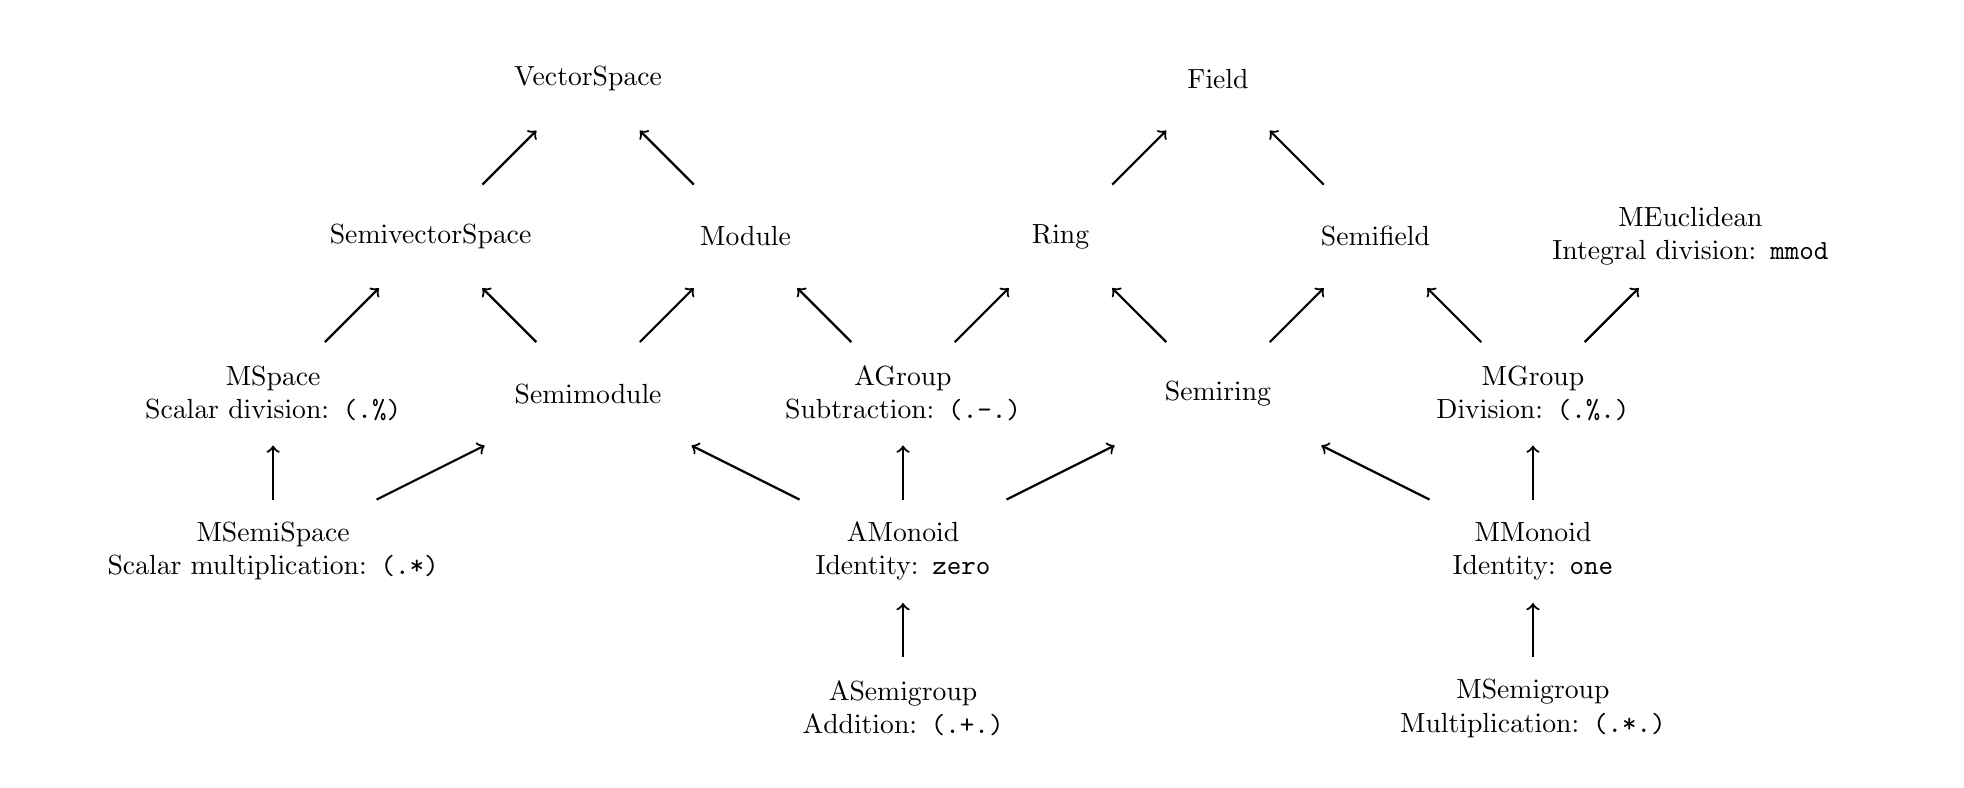
\begin{tikzpicture}
  % additive
  \node[plain] (asemigroup) at (8,0) {\bftt{ASemigroup} \\ Addition: \texttt{(.+.)}};
  \node[plain] (amonoid)    at (8,2) {\bftt{AMonoid} \\ Identity: \texttt{zero}};
  \node[plain] (agroup)     at (8,4) {\bftt{AGroup} \\ Subtraction: \texttt{(.-.)}};
  \draw[thick, ->] (asemigroup) -- (amonoid);
  \draw[thick, ->] (amonoid)    -- (agroup);

  % multiplicative
  \node[plain] (msemigroup)      at (16,0) {\bftt{MSemigroup} \\ Multiplication: \texttt{(.*.)}};
  \node[plain] (mmonoid)         at (16,2) {\bftt{MMonoid} \\ Identity: \texttt{one}};
  \node[plain] (mgroup)          at (16,4) {\bftt{MGroup} \\ Division: \texttt{(.\%.)}};
  \node[plain] (meuclidean)  at (18,6) {\bftt{MEuclidean} \\ Integral division: \texttt{mmod}};
  \draw[thick, ->] (msemigroup) -- (mmonoid);
  \draw[thick, ->] (mmonoid)    -- (mgroup);
  \draw[thick, ->] (mgroup)    -- (meuclidean);

  % semiring
  \node[plain] (semiring) at (12,4) {\bftt{Semiring}};
  \draw[thick, ->] (amonoid) -- (semiring);
  \draw[thick, ->] (mmonoid) -- (semiring);

  % ring and semifield
  \node[plain] (ring)      at (10,6) {\bftt{Ring}};
  \node[plain] (semifield) at (14,6) {\bftt{Semifield}};
  \draw[thick, ->] (agroup)   -- (ring);
  \draw[thick, ->] (semiring) -- (ring);
  \draw[thick, ->] (mgroup)   -- (semifield);
  \draw[thick, ->] (semiring) -- (semifield);

  % field
  \node[plain] (field)  at (12,8) {\bftt{Field}};
  \draw[thick, ->] (ring)      -- (field);
  \draw[thick, ->] (semifield) -- (field);

  % msemispace and mspace
  \node[plain] (msemispace) at (0,2) {\bftt{MSemiSpace} \\ Scalar multiplication: \texttt{(.*)}};
  \node[plain] (mspace)     at (0,4) {\bftt{MSpace} \\ Scalar division: \texttt{(.\%)}};
  \draw[thick, ->] (msemispace) -- (mspace);

  % semimodule
  \node[plain] (semimodule) at (4,4) {\bftt{Semimodule}};
  \draw[thick, ->] (msemispace) -- (semimodule);
  \draw[thick, ->] (amonoid)    -- (semimodule);

  % module and semivectorspace
  \node[plain] (module)          at (6,6) {\bftt{Module}};
  \node[plain] (semivectorspace) at (2,6) {\bftt{SemivectorSpace}};
  \draw[thick, ->] (agroup)     -- (module);
  \draw[thick, ->] (semimodule) -- (module);
  \draw[thick, ->] (semimodule) -- (semivectorspace);
  \draw[thick, ->] (mspace)     -- (semivectorspace);

  %vectorspace
  \node[plain] (vectorspace) at (4,8) {\bftt{VectorSpace}};
  \draw[thick, ->] (module)          -- (vectorspace);
  \draw[thick, ->] (semivectorspace) -- (vectorspace);
\end{tikzpicture}

\end{document}
